\chapter{Robust Command Arbitration for Modular Reinforcement Learning}

In this chapter I present a novel contribution to MRL.

\section{Modular reinforcement learning}

A second kind of decomposition in reinforcement learning, which is somewhat confusingly referred to as modular reinforcement learning (MRL) ~\cite{russell2003q-decomposition,sprague2003multiple-goal}, decomposes the original problem concurrently rather than temporally. In contrast to HRL, current MRL implementations do not involve delegation; instead, an agent is decomposed into several components, each of which is concurrently learning a subgoal of the original, complex, multiple-goal learning problem. On each occasion that a decision for what action to take is needed, an arbitrator combines the action preferences of the components to compute the output of the joint policy.  The current state of the art in modular reinforcement learning uses the the Q-values of the components directly to effect the arbitration decision.  Russell's and Zimdars's Q-decomposition \cite{russell2003q-decomposition} views the problem as a value function decomposition.  Sprague and Ballard view the problem more explicitly as arbitration, that is, action selection among multiple concurrently executing modules, although their solution, Greatest-Mass (GM) Sarsa \cite{sprague2003multiple-goal} is equivalent to Q-decomposition.

We would like these components to be truly modular. In particular, we would like the components to be reusable and easily understood by agent authors.  Unfortunately, current approaches implicitly require a global, monolithic reward signal, which detracts from these properties.  In particular, it detracts from the ability of the agent author to locally define the reward for a component.

Because the terms {\em hierarchical} and {\em modular} are often vague and overloaded, we use HRL to denote {\em temporally decomposable
  reinforcement learning} and MRL to denote {\em concurrently
  decomposable reinforcement learning}.

\subsection{Command Arbitration}

Like any software engineering, agent programming would benefit from modularity.  Truly modular reinforcement learning would facilitate speed of learning convergence, state abstraction, and transfer -- a component that has learned in one context can be reused (including its learned policy) in another context because the component is dependent only on its own local reward signal.  In this section we discuss the difficulties that current approaches face in achieving true modularity and present a new formulation which solves the core problem in Section \ref{sec:mrl-solution}.

To properly investigate our proposed mechanism of combining local learners, we will restrict our attention to the MRL framework. In this framework, a learning agent, $M$, is represented by a set of $n$ subproblems (components), $M=\{M_j\}_{j=1}^n$, each having its own reward signal and state space. The typical formulation is to have subproblems share an action set, thus $M_j = (S_j,A,R_j)$. When the agent takes an action in the world, each subproblem's state is updated, and each subproblem receives a reward. The agent can be thought of as having a state space that is a cross product of the subproblem state spaces, $S=S_1\times S_2\times\ldots\times S_n$. Traditionally, it is assumed that the agent's reward is a sum of subproblem rewards, $R(s,a)=\sum_{j\in N} R_j(s,a)$, where $N=\{1,\ldots,n\}$. Thus, $M$ is well-defined as a reinforcement learning problem, $M=(S,A,R)$, and the goal is to find a joint policy $\pi(s)$, composed of locally learned policies $\pi_j(s)$, that is optimal for the whole agent. We let $Q_j(s,a)$ refer to the Q-value learned by component $j$ for state $s$ and action $a$. Again, traditionally, $Q(s,a)=\sum_{j\in N} Q_j(s,a)$.

\subsection{Merging local signals}

Difficulty arises when multiple single goals are being combined in a larger, multi-goal learning problem. Take AvoidWolf and FindFood for instance; it is fairly straightforward to code an internally consistent reward signal for each.  However, it is unclear how to combine the two into the larger task of LiveLong.  For example, if there is no penalty for failing to eat within a certain time period (starvation), then the obvious policy is to avoid the predator and ignore the food.  Such a degenerate case could also happen if the reward signal for one learning module were scaled without re-engineering the other reward signals in the system, a problem dealt with by Bhat, et., al. \cite{bhat2006on-the-difficulty}.  For example, one could imagine swapping-in a new AvoidWolf module with a reward several times higher than the previous module, such that avoiding the predator always carries higher reward than finding the food.  In this case, a delegating agent would favor AvoidWolf to the near exclusion of FindFood.  The ability to substitute learning modules without modifying the rest of the system is one of the primary benefits of true modularity, and this modularity is difficult to achieve if local reward signals must be merged.


\subsection{Ideal Arbitration is Impossible}

Aside from the practical challenges cited above, Bhat, et., al. \cite{bhat2006on-the-difficulty} \cite{bhat2006on-the-difficulty} showed that ideal arbitration is impossible in full generality because command arbitration reduces to Arrow's Paradox \cite{arrow1963social}: an agent is a ``society'' of subagents, and command arbitration is social choice.  The problem is that we want the arbitrator to have the following reasonable properties:

\begin{itemize}

\item \textbf{Universality}: the ability to handle any possible set of
  subagents.

\item \textbf{Unanimity}: guarantee that if every subagent prefers
  action A, so will the arbitrator.

\item \textbf{Independence of Irrelevant Alternatives}: each
  subagent's preference for actions A and B are independent of the
  availability of any other action C, prevents any particular
  subagent from affecting the global action choice by dishonestly
  reporting its own preference ordering.

\item \textbf{Scale Invariance}: ability to scale any subagent's
  Q-values without affecting the arbitrator's choice.  This is the
  crucial property that allows separately authored subagents with
  incomparable reward signals.

\item \textbf{Non-Dictatorship}: no subagent gets its way all the time.

\end{itemize}

According to Arrow's Paradox, if $|A|\geq 3$, then there does not exist an arbitration function that satisfies each of the properties listed above.  So even simple agents are too complex for theoretically ideal arbitration.  This dissertation contributes a novel formulation of MRL and an algorithm that implements it, which we discuss in Section \ref{sec:mrl-arbiq}.

\section{Reformulating MRL}

Bhat, et., al., \cite{bhat2006on-the-difficulty} argued for a ``benevolent dictator'' arbitrator function but left the arbitration algorithm unspecified.  The contribution of this work is to show that a first-cut arbitration algorithm embodying the ideas in \cite{bhat2006on-the-difficulty} performs competitively with other MRL algorithms and shows superior robustness to subagent modification.  This robustness to subagent modification is the chief enabler of truly modular reinforcement learning in which subagents can be transferred from one system to another without having to re-engineer the reward signals to fit the new host system.

%% In this work, we relax the dictatorship requirement in order to make a
%% practical arbitrator-based learning algorithm feasible.  In the next
%% section we present our Arbi-Q algorithm based on this practicalized
%% arbitrator-based framework.

%% This is a ``fix'' because it is a reformulation. It doesn't get around
%% the impossibility result but instead defines a different thing to
%% optimize.  This fits though...now all learners are more homogenous;
%% they all have a local reward signal to optimize.

%% So while it is hard to write once-and-for-all a reward signal for a
%% multiple-goal learning problem, it is easier to write a collection of
%% single-goal reward signals, and hopefully combine them in a meaningful
%% way. Whereas in previous work, we show that there is no
%% general-purpose arbitration rule for combining subgoal preferences, in
%% the present work we make the hypothesis that the arbitrator itself is
%% a subgoal and thus has it's own notion of what it means to do its
%% subgoal well, i.e, has it's own reward signal. This means, given the
%% appropriate state, the supergoal can learn to select substeps
%% optimally. The question is what state constitutes ``appropriate
%% state''. The uninteresting case is the one in which the supergoal
%% state is simply the world state, in which case we have garnered no
%% saving, as this is simply flat RL all over again.

%In discussing MRL techniques, we will follow the nomenclature as
%introduced by ~\cite{sprague03multiple}.

\subsection{Formalization}

Our reformulation of MRL adds an {\em arbitrator} \cite{brooks1986a-robust}.  The arbitrator has a state space that may the same as or different from the subagents' state spaces, an action set that represents choosing a subagent, $A_0 = {1 ... n}$, and a reward signal that represents the ``greater good.''

The agent's policy is defined indirectly by the arbitrator's policy, $\pi_0(s, a)$, which assigns probabilities to the selection of each subagent's preferred action for each state.  This formulation relaxes the non-dictatorship requirement of ideal arbitration if you think of the arbitrator as a special subagent.  By Arrow's theorem, other properties will still hold.

For the agent author, this formulation adds the requirement of authoring a dedicated reward signal for the arbitrator.  For our bunny agent, this is LiveLongProsper:

\begin{itemize}
\item {\em Why} avoid predator, {\em why} eat? To live longer.
\item Encodes the tradeoffs between subagents -- perhaps food is more
  important to some bunnies.
\item The arbitrator could be hand-authored, or could be another RL
  agent.
\end{itemize}

For the small cost of authoring a reward signal that represents the ``greater good'' you get true modularity, that is, the ability to combine separately authored subagents with incomparable rewards.  This new reward signal is now the metric we use to measure the performance of the agent.

\section{The Arbi-Q Command Arbitration Algorithm}\label{sec:mrl-arbiq}

Formally, all we have changed in the traditional MRL formulation from Section \ref{sec:mrl-problem} is that $R(s,a)$ is now independently defined rather than being derived from the subgoal rewards.  It is now another part of the problem specification; in the partial programming setting, this corresponds to $R(s,a)$ being human-authored.  The solution to a MRL problem is a policy $\pi(s)$ which maximizes the long-term expected discounted reward under the arbitrator's reward $R(s,a)$.

Note that now $R(s,a)$ may or may not be equal to the sum of the rewards of its subgoals.  In fact, the subgoal rewards $R_j(s,a)$ may not have any correlation with the arbitrator's reward $R(s,a)$.

Arbi-Q uses the standard Q-Learning algorithm to learn a policy for choosing which of its $n$ subagents to delegate the task of selecting actions from $A$.  The arbitrator's action set $\widehat{A}$ is distinct from the set of primitive actions $A$.  To choose a primitive action to finally effect in the world, the agent first computes which subagent to delegate to, $j=\widehat{\pi}(\widehat{s})$, and then selects the primitive action given by the policy for subgoal $j$, namely $a=\pi_j(s_j)$, where $s_j \in S_j$.

\section{Experiments}

Our principal claim is that Arbi-Q is robust to subagent modification.  Our experiments will show that GM-Q/Q-decomposition degrades when a subagent is modified to have an incomparable reward signal and that Arbi-Q is robust to such modification.

\subsection{Bunny-Wolf World}

We use a world derived from Sprague and Ballard ~\cite{sprague2003multiple-goal}.  In Bunny-Wolf world, our agent is a bunny that must eat food and avoid being eaten by a wolf.  We can represent such an agent in our formulation as follows:

\begin{itemize}

\item Agent's overall goal (implemented in arbitrator):
  LiveLongProsper.  For a given agent, being happy can mean dying
  young with a full stomach, or dying old but less sated.  Either
  conception of happiness requires the FindFood and AvoidWolf
  subagents defined below.  The arbitrator, in a sense, encodes the
  agent's ``value system'' by representing the relative weight the
  agent assigns to its subagents.

\item Subagent 1: FindFood.  The bunny agent must find food in order
  to continue living.  If an agent does not find food within some
  number of time steps, it starves, terminating the episode.

\item Subagent 2: AvoidWolf.  The bunny agent must avoid the wolf.
  Meeting the wolf terminates the episode.

\end{itemize}

\subsection{Methodology}

%Show the update equations (Q-learning, Sarsa, gradient Sarsa)...with
%references.

We validate Arbi-Q's performance by comparing it with Greatest Mass Sarsa, which is a Q-decomposition algorithm that orders actions by their summed Q-value, $X_a=\sum_j Q_j(s,a)$. The arbitrator then selects the action with the largest $X_a$ value (the one with the
  ``greatest mass'').

We evaluate each algorithm similarly to Sprague and Ballard \cite{sprague2003multiple-goal} by training for 100,000 time steps and evaluating performance every 10,000 steps.  Performance is evaluated by running the greedy policy in the world for 1000 episodes and calculating the average reward per episode.  Each algorithm used a discount rate of 0.9 and $\epsilon$-greedy action selection during training.

For baselines, GM and Arbi-Q algorithms used subagents with similarly scaled rewards.  Unlike the Predator world from Sprague and Ballard \cite{sprague2003multiple-goal}, our FindFood subagent reaches a terminal state (death by starvation) after a fixed number of time steps.  This modification forces the agent to pursue both subgoals simultaneously in order to achieve long life.  In previous work the agent could achieve long life by avoiding the predator to the exclusion of finding food.

For robustness validation, we scaled the FindFood subagent reward by 10 to simulate the swapping out of separately-authored learning modules.  We believe that a truly modular arbitrator function should handle such subagent modification without serious degradation of performance.  Otherwise, any time a learning module were modified, the arbitrator, and possibly all the other modules, would need to be modified to ensure compatibility.

\section{Results}

\begin{figure}[ht]
  \begin{center}
    \scalebox{.75}{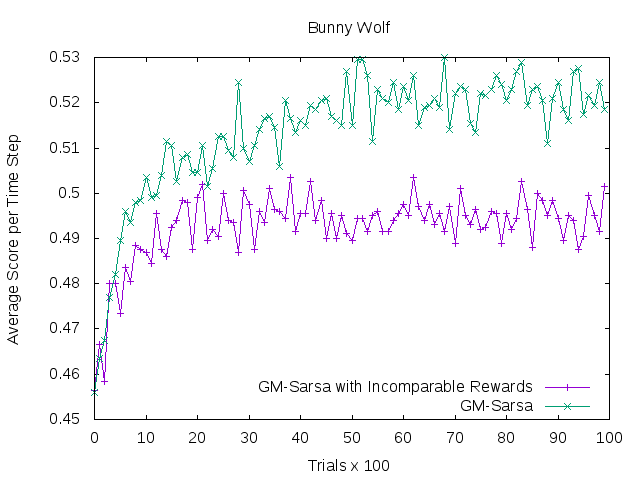
\includegraphics{gm-bunny-wolf.png}}
    \scalebox{.75}{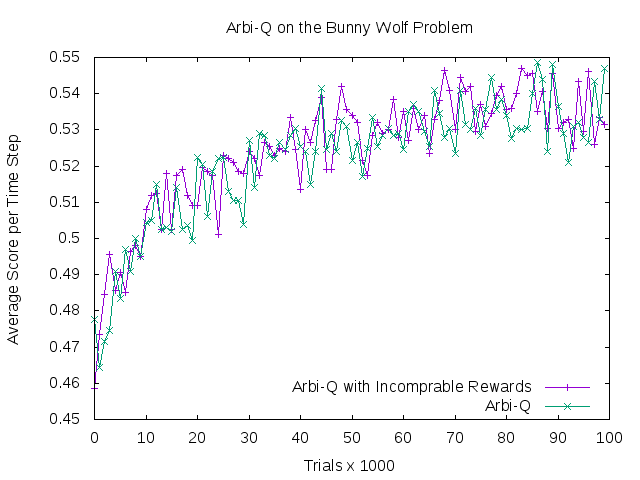
\includegraphics{arbiq-bunny-wolf.png}}
    \caption{Performance of Arbi-Q versus GM-Sarsa/Q-decomposition on the bunny-wolf problem. The top plot shows that Greatest Mass command arbitration degrades significantly when its subagent rewards are incomprable. Arbi-Q shows no degredation in performance when subagents have incomprable rewards, suggesting that it is amenable to ``swappable'' subagents.}
  \end{center}
  \label{fig:gmresults}
\end{figure}


\section{Discussion}
